% ==============================================================================
% LAB 119
% UNDERSÖKNING AV RC-KRETS
% ------------------------
%
% Author:
% Jonas Sjöberg     <tel12jsg@student.hig.se>
% Oscar Wallberg    <tco13owg@student.hig.se>
%
% License:
% Creative Commons Attribution-NonCommercial-ShareAlike 4.0 International
% See LICENSE.md for full licensing information.
% ==============================================================================

\section{Inverkan av källimpedans och belastningsimpedans}\label{impedans}
% ------------------------------------------------------------------------------
% Hittills har vi inte tagit hänsyn till hur signalgeneratorns och oscilloskopets
% impedanser kan påverka funktionen hos vår krets. Ett mera fullständigt schema
% över vår uppkoppling ser ut så här:
% 
% Om vi betraktar kondensatorn som kortsluten för höga frekvenser och som helt
% öppen för låga frekvenser så inser vi lätt att inimpedansen för RC-filtret Zin
% 1k och utimpedansen Zut 1k. Det är alltså rimligt att anta att varken
% signalgeneratorns eller oscilloskopets impedanser inverkar nämnvärt på kretsens
% funktion i vår uppkoppling.  Men vad händer om vi har käll- eller
% belastningsimpedanser i samma storleksordning som RC-kretsens egna impedanser?
% Vi kan undersöka detta genom att ansluta motstånd på in- och utgången av
% kretsen.

\section{Inverkan av källimpedansen}\label{Zin}
% ------------------------------------------------------------------------------
% För att se hur kretsen uppför sig om vi ansluter den till en signalgenerator
% med utimpedansen 1k (dvs egentligen 1k + 50) kopplar vi upp följande krets:

% TODO: Lägg till Kopplingsschema


\subsection{Mätresultat}\label{}
% ------------------------------------------------------------------------------
% TODO: Mät upp Bode-diagrammet för kretsen och jämför med tidigare fall, 
%       vi nöjer oss med amplituddiagrammet i denna mätning. 
%       Notera brytfrekvensen. 
%       Uin är den "nya" funktionsgeneratorns utspänning utan belastning.

% TODO: Lägg till signalgeneratorns amplitud vid mätning.
$U_{in} = 1 \si{\volt}$

% TODO: Lägg till faktiska mätresultat i tabellen.
\begin{longtable}[c]{@{}ccccc@{}}
  \toprule\addlinespace
    \begin{tabular}{cc}$\text{Frekvens}        \\ (\si{\hertz})$   \end{tabular}
  & \begin{tabular}{cc}$U_{ut}                 \\ (\si{\volt})$    \end{tabular}
  & \begin{tabular}{cc}$U_{ut}/U_{in}          \\ (\si{\volt})$    \end{tabular}
  & \begin{tabular}{cc}$20 \log{U_{ut}/U_{in}} \\ (\si{\dB})$      \end{tabular}
  \\\addlinespace
  \midrule\endhead
   100 & 2.11 & 1.01 & 5   \\\addlinespace
   200 & 2.06 & 0.99 & 10  \\\addlinespace
   300 & 2    & 0.96 & 17  \\\addlinespace
   500 & 1.94 & 0.93 & 24  \\\addlinespace
   700 & 1.84 & 0.88 & 29  \\\addlinespace
  1000 & 1.75 & 0.84 & 33  \\\addlinespace
  1200 & 1.66 & 0.79 & 37  \\\addlinespace
  1300 & 1.56 & 0.75 & 42  \\\addlinespace
  1500 & 1.49 & 0.71 & 45  \\\addlinespace
  1700 & 1.39 & 0.67 & 49  \\\addlinespace
  2000 & 1.39 & 0.67 & 49  \\\addlinespace
  \bottomrule
  \addlinespace
  \caption[]{Mätresultat för kretsen i Figur~\ref{fig:rc-schema}.}
  \label{8a-table}
\end{longtable}

% TODO: Bode-diagram för frekvensgång (amplitud vs frekvens).

% TODO: Hur påverkas amplituden och brytfrekvensen av källimpedansen? 


\section{Inverkan av belastningsimpedansen}\label{Zut}
% ------------------------------------------------------------------------------
% För att undersöka hur kretsen påverkas av en belastning på 1k kopplar vi upp
% följande:

% TODO: Lägg till Kopplingsschema


\subsection{Mätresultat}\label{}
% ------------------------------------------------------------------------------
% TODO: Mät upp amplituddiagrammet och notera brytfrekvensen.

% TODO: Lägg till signalgeneratorns amplitud vid mätning.
$U_{in} = 1 \si{\volt}$

% TODO: Lägg till faktiska mätresultat i tabellen.
\begin{longtable}[c]{@{}ccccc@{}}
  \toprule\addlinespace
    \begin{tabular}{cc}$\text{Frekvens}        \\ (\si{\hertz})$   \end{tabular}
  & \begin{tabular}{cc}$U_{ut}                 \\ (\si{\volt})$    \end{tabular}
  & \begin{tabular}{cc}$U_{ut}/U_{in}          \\ (\si{\volt})$    \end{tabular}
  & \begin{tabular}{cc}$20 \log{U_{ut}/U_{in}} \\ (\si{\dB})$      \end{tabular}
  \\\addlinespace
  \midrule\endhead
   100 & 2.11 & 1.01 & 5   \\\addlinespace
   200 & 2.06 & 0.99 & 10  \\\addlinespace
   300 & 2    & 0.96 & 17  \\\addlinespace
   500 & 1.94 & 0.93 & 24  \\\addlinespace
   700 & 1.84 & 0.88 & 29  \\\addlinespace
  1000 & 1.75 & 0.84 & 33  \\\addlinespace
  1200 & 1.66 & 0.79 & 37  \\\addlinespace
  1300 & 1.56 & 0.75 & 42  \\\addlinespace
  1500 & 1.49 & 0.71 & 45  \\\addlinespace
  1700 & 1.39 & 0.67 & 49  \\\addlinespace
  2000 & 1.39 & 0.67 & 49  \\\addlinespace
  \bottomrule
  \addlinespace
  \caption[]{Mätresultat för Inverkan av belastningsimpedansen för kretsen i Figur~\ref{fig:rc-schema}.}
  \label{8a-table}
\end{longtable}


% TODO: Bode-diagram för frekvensgång (amplitud vs frekvens).

% TODO: Hur påverkas amplituden och brytfrekvensen av belastningsimpedansen? 
%       Förklara vad som händer!



\subsection{Simulering}\label{}
% ------------------------------------------------------------------------------
Kretsen simuleras i \texttt{Qucs} enligt Figur~\ref{fig:Zin-step} och
Figur~\ref{fig:Zout-step}.

Källimpedansens påverkar på kretsen kan ses i Figur~\ref{fig:Zin-step} som
visar kretsens frekvensrespons då värdet av $R_i$ sveps mellan $\SI{50}{\ohm}$
och $\SI{10}{\kohm}$ i $20$ steg om $\SI{523.684}{\ohm}$.

Påverkan från belastningsimpedansen ses i Figur~\ref{fig:Zout-step} som visar
kretsens frekvensrespons då värdet av $R_o$ sveps mellan $\SI{100}{\ohm}$ och
$\SI{1}{\mega\ohm}$ i $101$ steg om $\SI{9.999}{\kohm}$.


\begin{figure}[ht]\label{fig:Zin-step}
  \centering
  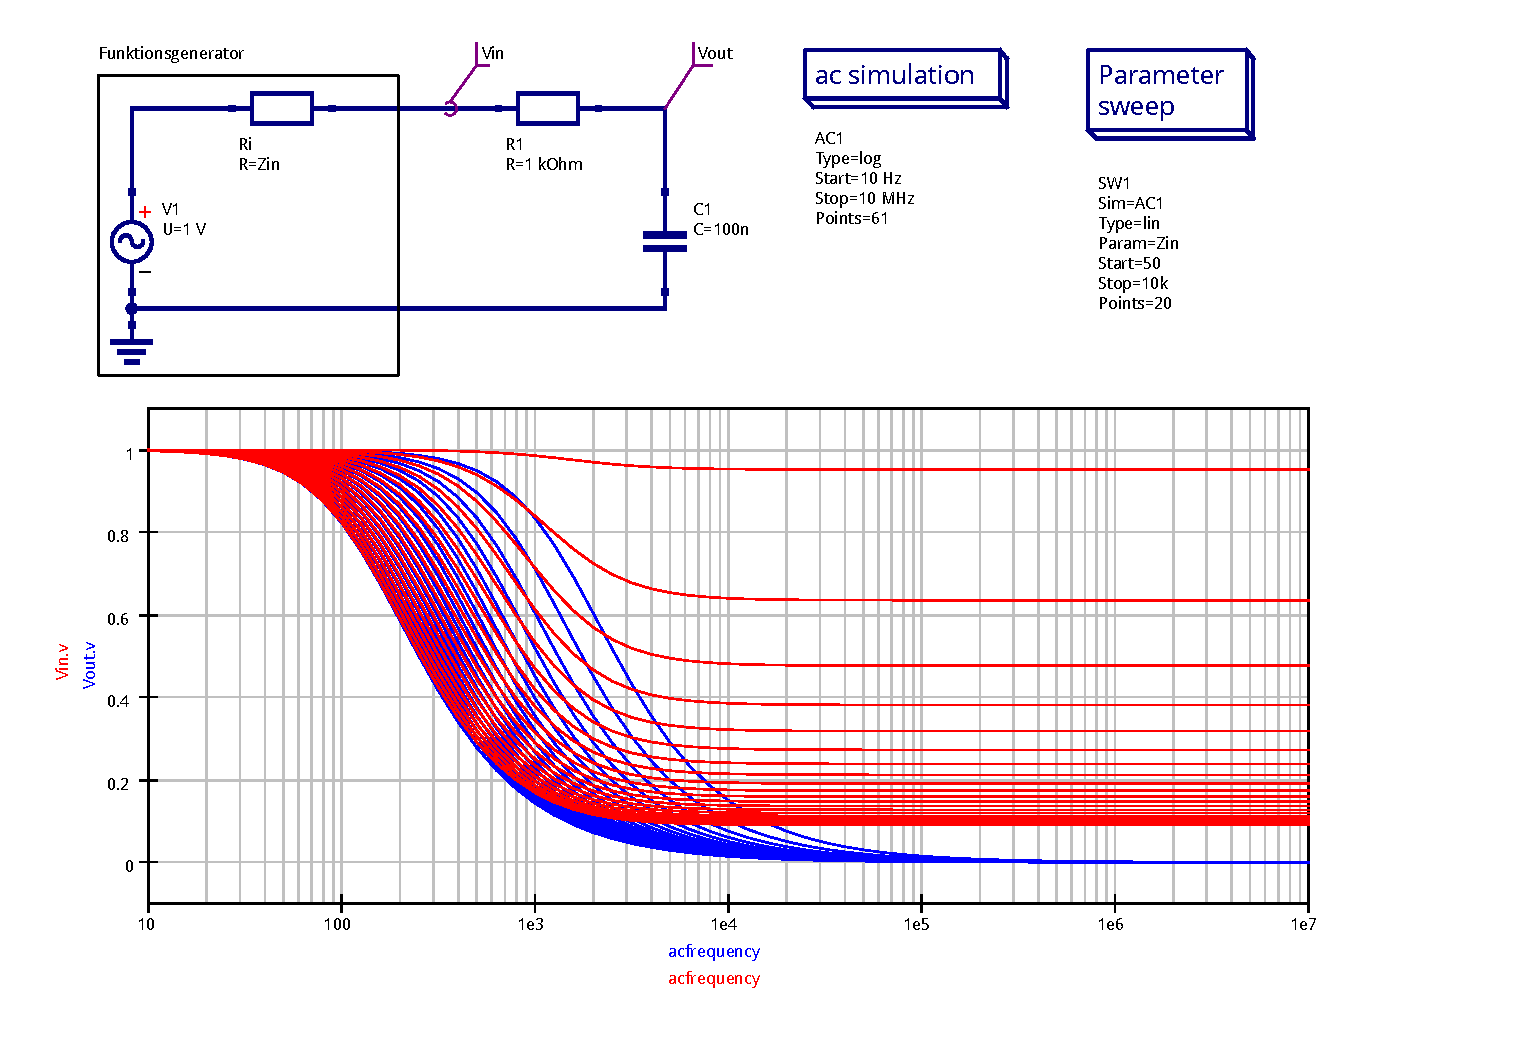
\includegraphics[width=\linewidth]{sim/ee466_lab-4_prj/uppgift-3_Zin_step}
  \caption[] {Simulering av kretsens frekvensrespons för olika värden av $R_i$.}
\end{figure}

\begin{figure}[ht]\label{fig:Zout-step}
  \centering
  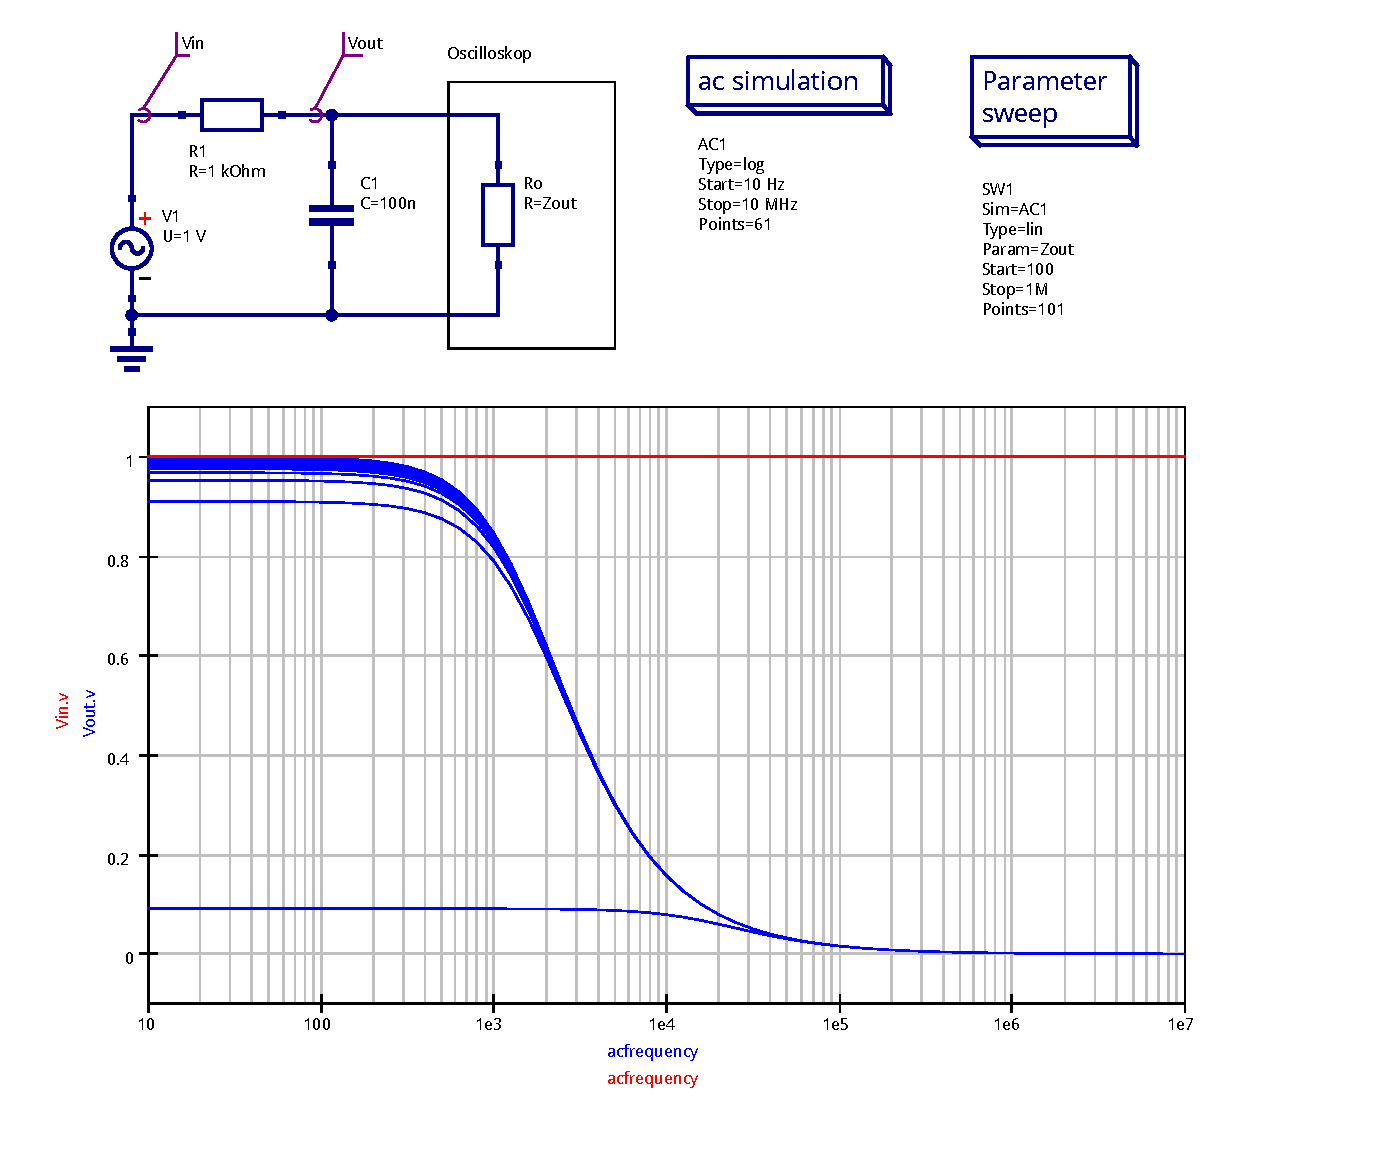
\includegraphics[width=\linewidth]{sim/ee466_lab-4_prj/uppgift-3_Zout_step}
  \caption[] {Simulering av kretsens frekvensrespons för olika värden av $R_o$.}
\end{figure}

\subsection{Kommentar}\label{}
% ------------------------------------------------------------------------------
% TODO:


